\documentclass[t]{beamer}
\usepackage[
    orientation=landscape,
    size=custom,
    width=25.4,
    height=19.05,
    scale=0.63 % erzeugt 16pt Schriftgröße
]{beamerposter}

\newcommand{\PraesentationSchriftgroesseSehrGross}{\fontsize{30}{45}}
\newcommand{\PraesentationSchriftgroesseGross}{\fontsize{22}{33}}
\newcommand{\PraesentationSchriftgroesseNormal}{\fontsize{16}{29}}
\newcommand{\PraesentationSchriftgroesseKlein}{\fontsize{12}{18}}
\newcommand{\PraesentationSchriftgroesseDreizeiler}{\fontsize{7}{10}}
\newcommand{\PraesentationSchriftgroesseAufzaehlungszeichen}{\fontsize{10}{8}}

\newcommand{\PraesentationAbstandAbsatz}{22.1pt}
\newcommand{\PraesentationPositionKorrekturOben}{-1.8cm}
\newcommand{\PraesentationBeispieleSchriftgroessen}{30 | 22 | 16 | 12}

\usepackage[ascii]{inputenc}
%\usepackage[T1]{fontenc} % Zeichensatzkodierung

\usepackage{upquote}

\usepackage{calc} % Berechnungen

\usepackage[english]{babel}
\usepackage{graphicx}
\usepackage[caption=false]{subfig}
\usepackage[export]{adjustbox}
\usepackage[absolute, overlay]{textpos} % Positionierung

% Silbentrennung:
\usepackage{hyphenat}

% Euro-Symbol:
\usepackage[gen]{eurosym}
\DeclareUnicodeCharacter{20AC}{\euro{}}

% Schriftart Helvetica:
\usepackage[scaled]{helvet}
\renewcommand{\familydefault}{\sfdefault}

\usepackage{mathptmx} % skalierbare Formelschriften

\usepackage{tabularx}

\usepackage{multicol} % mehrspaltiger Text

\usepackage{csquotes}

\usepackage{tikz}
\usetikzlibrary{arrows, shapes, shapes.multipart, trees, positioning, backgrounds, fit, matrix, calc, patterns}

% Diagramme:
%\usepackage{pgfplots}
%\pgfplotsset{compat=default}

\usepackage[
    style=authoryear-comp,
    bibstyle=authoryear,
    maxnames=2,
    giveninits=true,
    uniquename=init,
    doi=false
]{biblatex}

\DeclareNameAlias{sortname}{family-given}
\addbibresource{references.bib}

\usepackage{algorithm}
\usepackage[noend]{algpseudocode}

% within algorithmic
\makeatletter
\let\OldStatex\Statex
\renewcommand{\Statex}[1][3]{%
    \setlength\@tempdima{\algorithmicindent}%
    \OldStatex\hskip\dimexpr#1\@tempdima\relax}
\makeatother

% Erweiterbare Fusszeile:
\newcommand{\PraesentationFusszeileZusatz}{}


\newcommand{\R}{{\mathbb{R}}}
\newcommand{\C}{{\mathbb{C}}}

\newcommand{\ud}{\mathrm{d}}

\newcommand{\ket}[1]{{\left\lvert{#1}\right\rangle}}

\DeclareMathOperator{\e}{e}
\DeclareMathOperator{\tr}{tr}
\DeclareMathOperator*{\argmin}{argmin}
\DeclareMathOperator*{\argmax}{argmax}

\graphicspath{{figures/}}


% Für die Person anpassen:
\newcommand{\PersonTitel}{}
\newcommand{\PersonVorname}{Christian B.}
\newcommand{\PersonNachname}{Mendl}

% Fakultät:
\newcommand{\FakultaetName}{Department of Informatics 5}
\newcommand{\LehrstuhlName}{Chair of Scientific Computing in Computer Science (SCCS)}

\newcommand{\Datum}{March 10, 2020}

\renewcommand{\PraesentationFusszeileZusatz}{| Reinforcement Learning}

\title{Reinforcement Learning Introduction}
\author{\PersonTitel{} \PersonVorname{} \PersonNachname}
\institute[]{\UniversitaetName \\ \FakultaetName \\ \LehrstuhlName}
\date[\Datum]{March 10, 2020 \\ $ $ \\ {\color{TUMBlau} \href{https://github.com/cmendl/reinforcement-learning-course}{https://github.com/cmendl/reinforcement-learning-course}}}


% Allgemein:
\newcommand{\AllgemeinGestalter}{ediundsepp Gestaltungsgesellschaft}
\newcommand{\AllgemeinErsteller}{eWorks GmbH}

% Universität:
\newcommand{\UniversitaetName}{Technische Universit\"at M\"unchen}
\newcommand{\UniversitaetAbkuerzung}{TUM}
\newcommand{\UniversitaetWebseite}{www.tum.de}
\newcommand{\UniversitaetLogoBreite}{19mm}
\newcommand{\UniversitaetLogoHoehe}{1cm}

\newcommand{\PraesentationSeitenrand}{8.9mm}
\newcommand\crule[3][black]{\textcolor{#1}{\rule{#2}{#3}}}

\newlength\smallerbaselineskip
\setlength{\smallerbaselineskip}{0.8\baselineskip}

    % Blautöne:
\definecolor{TUMBlau}{RGB}{0,101,189} % Pantone 300
\definecolor{TUMBlauDunkel}{RGB}{0,82,147} % Pantone 301
\definecolor{TUMBlauHell}{RGB}{152,198,234} % Pantone 283
\definecolor{TUMBlauMittel}{RGB}{100,160,200} % Pantone 542

    % Hervorhebung:
\definecolor{TUMElfenbein}{RGB}{218,215,203} % Pantone 7527 -Elfenbein
\definecolor{TUMGruen}{RGB}{162,173,0} % Pantone 383 - Grün
\definecolor{TUMOrange}{RGB}{227,114,34} % Pantone 158 - Orange
\definecolor{TUMGrau}{gray}{0.6} % Grau 60%


\setbeamercolor*{alerted text}{fg=TUMOrange}

\newcommand{\PraesentationSetzeTextfarbe}{%
    \color{PraesentationTextfarbe}%
    \setbeamercolor*{frametitle}{fg=PraesentationTextfarbe}%
    \setbeamercolor*{normal text}{fg=PraesentationTextfarbe}%
    \setbeamercolor{itemize/enumerate body}{fg=PraesentationTextfarbe}%
    \setbeamercolor*{itemize item}{fg=PraesentationTextfarbe}%
}

\newcommand{\PraesentationFarbschemaStandard}{%
    \setbeamercolor*{background canvas}{}%
    \definecolor{PraesentationTextfarbe}{rgb}{0,0,0}%
    \PraesentationSetzeTextfarbe%
}

\newcommand{\PraesentationFarbschemaWeissBlau}{%
    \setbeamercolor*{background canvas}{bg=TUMBlauDunkel}%
    \definecolor{PraesentationTextfarbe}{rgb}{1,1,1}%
    \PraesentationSetzeTextfarbe%
}

\newcommand{\PraesentationFarbschemaWeissSchwarz}{%
    \setbeamercolor*{background canvas}{bg=black}%
    \definecolor{PraesentationTextfarbe}{rgb}{1,1,1}%
    \PraesentationSetzeTextfarbe%
}

\newcommand{\PraesentationTitelseiteInhalt}{%
    \begin{textblock*}{\paperwidth}[0,0](0cm,-\PraesentationSeitenrand - 6.5mm + \PraesentationPositionKorrekturOben)%
        \color{PraesentationTextfarbe}%
        \frametitle{\inserttitle}
        \vspace*{49.4mm}%
        \usebeamerfont{author}\selectfont\insertauthor\\%
        \insertinstitute\\%
        \insertdate%
    \end{textblock*}%
}

\newcommand{\PraesentationSeitenkopfInhalt}[1]{%
    %\vspace*{31.7mm}%
    \begin{textblock*}{1.68cm}[1,0](\paperwidth - \PraesentationSeitenrand - \PraesentationSeitenrand, 0cm)%
        \includegraphics[width=1.68cm]{#1}%
    \end{textblock*}%
    \begin{textblock*}{3cm}[1,0](\paperwidth - \PraesentationSeitenrand, -\PraesentationSeitenrand)%
        \hbox{%
            \color{PraesentationTextfarbe}%
            \hbox{\insertframenavigationsymbol}%
            \hbox{\insertsubsectionnavigationsymbol}%
            \hbox{\insertsectionnavigationsymbol}%
        }%
    \end{textblock*}%
}

\newcommand{\PraesentationBildUhrenturm}{%
    \begin{textblock*}{10.82cm}[1,1](\paperwidth - \PraesentationSeitenrand - \PraesentationSeitenrand, \paperheight - 9mm)%
        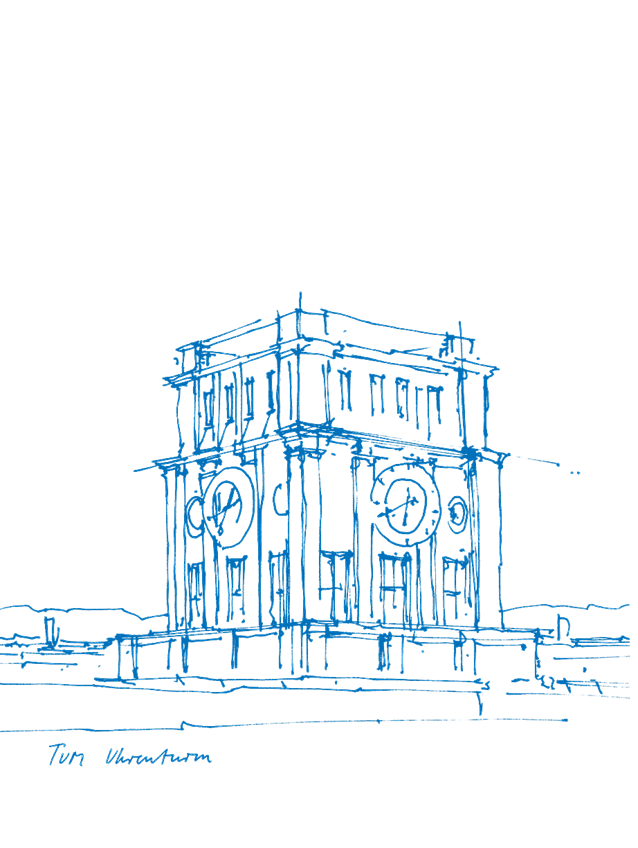
\includegraphics{TUM_Uhrenturm.png}%
    \end{textblock*}%
}

\newcommand{\PraesentationStartseiteUhrenturm}{%
    \setbeamertemplate{title page}{%
        \PraesentationSeitenkopfInhalt{Universitaet_Logo_RGB.pdf}%
        \PraesentationBildUhrenturm%
        \PraesentationTitelseiteInhalt%
    }%
}

\newcommand{\PraesentationStartseiteFlaggen}{%
    \setbeamertemplate{title page}{%
        \begin{textblock*}{\paperwidth}[0,1](-\PraesentationSeitenrand,\paperheight-\PraesentationSeitenrand)%
            
\includegraphics[min width=\paperwidth,max width=\paperheight,min totalsize={\paperwidth}{\paperheight},keepaspectratio,center]{Universitaet_Flaggen.jpg}%
        \end{textblock*}%
        \PraesentationSeitenkopfInhalt{Universitaet_Logo_weiss.pdf}%
        \PraesentationTitelseiteInhalt%
    }%
}

\newcommand{\PraesentationStartseiteLeer}{%
    \setbeamertemplate{title page}{%
        \PraesentationSeitenkopfInhalt{Universitaet_Logo_weiss.pdf}%
        \PraesentationTitelseiteInhalt%
    }%
}


\newcommand{\PraesentationMasterStandard}{%
    \PraesentationFarbschemaStandard%
    \PraesentationStartseiteUhrenturm%
    \setbeamertemplate{headline}{%
        \PraesentationSeitenkopfInhalt{Universitaet_Logo_RGB.pdf}%
    }%
}

\newcommand{\PraesentationMasterWeissBlau}{%
    \PraesentationFarbschemaWeissBlau%
    \PraesentationStartseiteLeer%
    \setbeamertemplate{headline}{%
        \PraesentationSeitenkopfInhalt{Universitaet_Logo_weiss.pdf}%
    }%
}


\newcommand{\PraesentationMasterWeissSchwarz}{%
    \PraesentationFarbschemaWeissSchwarz%
    \setbeamertemplate{title page}{%
        \PraesentationTitelseiteInhalt%
        \PraesentationSeitenkopfInhalt{Universitaet_Logo_weiss.pdf}%
    }
    \setbeamertemplate{headline}{%
        \PraesentationSeitenkopfInhalt{Universitaet_Logo_weiss.pdf}%
    }
}

\newcommand{\PraesentationTitelseite}{\frame[plain]{\titlepage}}
\newcommand{\PraesentationUeberschriftZweizeilig}[2]{\frametitle{#1\\[8mm]#2}}

\setbeamersize{
    text margin left=\PraesentationSeitenrand,
    text margin right=\PraesentationSeitenrand
}

\setbeamertemplate{frametitle}{%
    {\rule{0pt}{42mm + \PraesentationPositionKorrekturOben}\PraesentationSchriftgroesseSehrGross\selectfont\insertframetitle\newline\vspace*{-6.7mm}}%
}

% Aufzählungen:
\newcommand{\PraesentationAufzaehlungEbeneEinsSymbol}{\raise2pt\hbox{\donotcoloroutermaths\usebeamercolor{itemize subitem}\PraesentationSchriftgroesseAufzaehlungszeichen$\bullet$}}
\newcommand{\PraesentationAufzaehlungEbeneZweiSymbol}{\raise1.25pt\hbox{\donotcoloroutermaths\usebeamercolor{itemize subitem}$-$}}
\setbeamertemplate{itemize items}[circle]
\setbeamertemplate{itemize subitem}[triangle]
\setbeamercolor{itemize subitem}{fg=black}
\setbeamerfont{itemize/enumerate subbody}{size=\normalsize}
\setbeamertemplate{itemize item}{\PraesentationAufzaehlungEbeneEinsSymbol}
\setbeamertemplate{itemize subitem}{\PraesentationAufzaehlungEbeneZweiSymbol{}}
%\addtolength{\leftmarginii}{16mm-2pt}%

\newenvironment{PraesentationAufzaehlung}
{%
    \vspace{-\baselineskip}%
    \begin{itemize}%
        \setlength{\itemsep}{0pt}%
        \setlength{\parskip}{0pt}%
        \setlength{\parsep}{0pt}%
        \addtolength{\itemindent}{-1ex}%
}{%
    \end{itemize}%
}


% PDF-Einstellungen:
\hypersetup{
    pdfstartview={Fit},
    pdfproducer={\AllgemeinErsteller},
    pdfcreator={\AllgemeinGestalter}
}

\textblockorigin{\PraesentationSeitenrand}{\PraesentationSeitenrand} % Ursprung für Positionierung

\setbeamerfont{footnote}{size=\PraesentationSchriftgroesseKlein}

\setbeamertemplate{footline}{
    \hbox{%
        \usebeamerfont{footnote}%
        \begin{beamercolorbox}[wd=.9\paperwidth]{}%
            \hspace*{\PraesentationSeitenrand}%
            \PersonTitel{} \PersonVorname~\PersonNachname~(\UniversitaetAbkuerzung) \PraesentationFusszeileZusatz{}%
        \end{beamercolorbox}%
        \begin{beamercolorbox}[wd=.1\paperwidth]{}%
            \insertframenumber{}%
            \raggedleft
            \hspace*{\PraesentationSeitenrand}%
        \end{beamercolorbox}%
        \vspace*{3.25mm}%
    }%
}

\setbeamertemplate{navigation symbols}{}

\begin{document}
\setlength{\baselineskip}{\PraesentationAbstandAbsatz}
\setlength{\parskip}{\baselineskip}



\PraesentationMasterStandard

\PraesentationTitelseite



\PraesentationMasterWeissBlau

\begin{frame}
\frametitle{Outline}
\begin{itemize}
\item Introduction and motivation
\item Theoretical framework
\begin{itemize}
\item Markov decision processes (MDPs)
\item Iterative ``dynamic programming'' algorithms
\item Deep reinforcement learning
\item Policy gradients
\end{itemize}
\item Hands-on example: simplified Pac-Man
\end{itemize}
\end{frame}
\PraesentationMasterStandard



\PraesentationMasterWeissBlau
\begin{frame}
\frametitle{Introduction and motivation}
\end{frame}
\PraesentationMasterStandard



\begin{frame}
\frametitle{Motivation}
Goal-oriented behavior in a complex, non-deterministic environment

Example autonomous driving: steer vehicle safely from A to B, ``environment'' consists of other vehicles, bikes, pedestrians, street signs, \dots

\begin{center}
\includegraphics[width=0.6\textwidth]{agent_environment/agent_environment}
\end{center}

\vfill

{\small
S.~Russell and P.~Norvig. \emph{Artificial Intelligence: A Modern Approach (3rd edition).} Prentice Hall (2009) \nocite{RussellNorvig} \\
R.~S.~Sutton and A.~G.~Barto. \emph{Reinforcement Learning: An Introduction (2nd edition).} MIT Press (2018) \nocite{SuttonBarto}
}
\end{frame}



\begin{frame}
\frametitle{Deepmind's AlphaGo}
\begin{center}

\includegraphics[width=0.45\textwidth]{all_systems_go}
\end{center}
\end{frame}



\begin{frame}
\frametitle{Deepmind's Alphastar}
Reinforcement learning to train an agent to play StarCraft II
\begin{center}
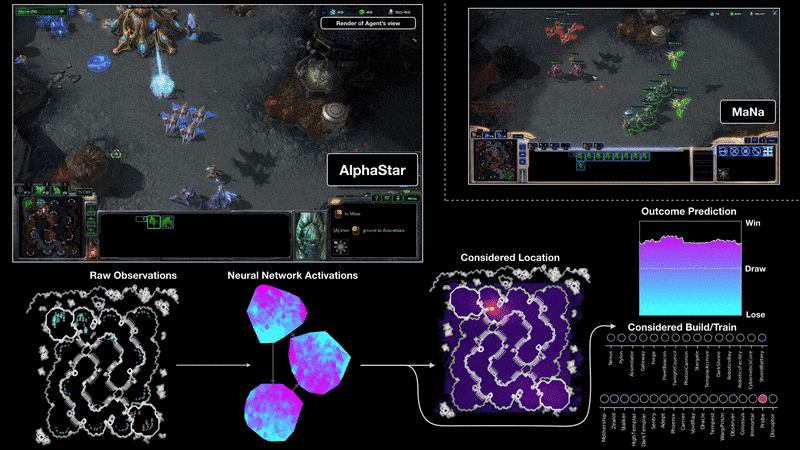
\includegraphics[width=0.85\textwidth]{alphastar_agent} \\
{\small
\href{https://deepmind.com/blog/article/alphastar-mastering-real-time-strategy-game-starcraft-ii}{https://deepmind.com/blog/article/alphastar-mastering-real-time-strategy-game-starcraft-ii}
}
\end{center}
\end{frame}



\PraesentationMasterWeissBlau
\begin{frame}
\frametitle{Theoretical framework}
\end{frame}
\PraesentationMasterStandard



\begin{frame}
\frametitle{MDPs: agent and environment}
Formal description: an agent interacts with an environment
\begin{figure}
\includegraphics[width=0.6\textwidth]{agent_environment/agent_environment}
\end{figure}

\textbf{State} of agent and environment at time points $t = 0, 1, 2, \dots$ denoted $s_t \in \mathsf{S}$

Agent chooses an \textbf{action} $a_t \in \mathsf{A}$ $\leadsto$ system transitions to next state $s_{t+1} \in \mathsf{S}$ with transition probability
\[
\mathbb{P}(s_{t+1} \vert s_t, a_t)
\]
\emph{Markov property}: probability does not explicitly depend on previous time points
\end{frame}



\begin{frame}
\frametitle{MDPs: reward and return}
At each time point the agent receives a \textbf{reward} (can be positive, zero or negative):
\[
r_t = R(s_t)
\]

Goal: maximize \textbf{return}: cumulative discounted reward
\[
\sum_{t=0}^\infty \gamma^t R(s_t), \quad 0 < \gamma \le 1
\]
with $\gamma^t$ the discount factor
\end{frame}



\begin{frame}
\frametitle{Model example: grid world}
$4 \times 3$ grid world with one player (hatched field $(2, 2)$ is inaccessible):
\begin{center}
\includegraphics[width=0.3\textwidth]{mdp_environment/mdp_environment}
\end{center}
\vspace{-0.5cm}
$s_t$: current actor (player) position

Possible actions: $\uparrow$, $\downarrow$, $\leftarrow$, $\rightarrow$: ``try to move in corresponding direction by one field''

\vfill

{\small
S.~Russell and P.~Norvig. \emph{Artificial Intelligence: A Modern Approach (3rd ed).} (2009) \nocite{RussellNorvig}
}
\end{frame}



\begin{frame}
\frametitle{Model example: grid world, continued}
Transition probability:
\begin{center}
\includegraphics[width=0.2\textwidth]{mdp_transition/mdp_transition}
\end{center}
Formally:
\begin{align*}
&\mathbb{P}\left( s_{t+1} = s_t + \left(\begin{smallmatrix} 0\\1\end{smallmatrix}\right) \vert s_t, a_t = \uparrow \right) = 0.8, \\
&\mathbb{P}\left( s_{t+1} = s_t + \left(\begin{smallmatrix} 1\\0\end{smallmatrix}\right) \vert s_t, a_t = \uparrow \right) = 0.1, \\
&\mathbb{P}\left( s_{t+1} = s_t + \left(\begin{smallmatrix}-1\\0\end{smallmatrix}\right) \vert s_t, a_t = \uparrow \right) = 0.1
\end{align*}
Analogously for $\downarrow$, $\leftarrow$, $\rightarrow$

Reward: $+1$ for exit field $(4,3)$, $-1$ for exit field $(4,2)$, $-0.04$ for any other field (agent wants to reach exit as fast as possible)

\vfill

{\small
S.~Russell and P.~Norvig. \emph{Artificial Intelligence: A Modern Approach (3rd ed).} (2009) \nocite{RussellNorvig}
}
\end{frame}



\begin{frame}
\frametitle{MDPs: policy function and utility}
How do we specify possible solutions?

Actions of agent specified by \textbf{policy} $\pi: \mathsf{S} \to \mathsf{A}$:
\[
a_t = \pi( s_t )
\]
Due to Markov property: only dependency on $s_t$ required (instead of full history $s_0, s_1, \dots, s_t$)

\pause

``Quality'' of $\pi$ quantified by \emph{expected return}, denoted \textbf{utility} or \textbf{value function}:
\[
U^\pi(s_0) = \mathbb{E}\!\left[ \sum_{t=0}^\infty \gamma^t R(s_t) \Big\vert \pi \right],
\]
$s_1, s_2, \dots$ now regarded as random variables

Notation $\mathbb{E}[\dots \vert \pi]$: use policy $\pi$ for choosing actions $a_t$
\end{frame}



\begin{frame}
\frametitle{Optimal policy and utility}
\[
\pi^* = \argmax_{\pi} U^\pi(s_0)
\]
$\pi^*$ does not depend on $s_0$! Justification: self-similar form:
\[
\mathbb{E}\!\left[ \sum_{t'=t}^\infty \gamma^{t'} R(s_{t'}) \Big\vert \pi, s_t = \tilde{s}_0 \right]
= \gamma^t \, \mathbb{E}\!\left[ \sum_{\Delta t=0}^\infty \gamma^{\Delta t} R(s_{t + \Delta t}) \Big\vert \pi, s_t = \tilde{s}_0 \right]
= \gamma^t \, U^\pi (\tilde{s}_0).
\]

Example (for $\gamma = 1$):
\begin{center}
\includegraphics[width=0.5\textwidth]{mdp_optimal_policy_example/mdp_optimal_policy_example}
\end{center}
\end{frame}



\begin{frame}
\frametitle{Optimal policy and utility, continued}
Corresponding value function for optimal policy: $U = U^{\pi^*}$ (omit superscript $\pi^*$)
\begin{center}
\includegraphics[width=0.3\textwidth]{mdp_optimal_value_example/mdp_optimal_value_example}
\end{center}

Conversely, can obtain $\pi^*$ from $U$:
\[
\pi^*(s) = \argmax_{a \in \mathsf{A}} \sum_{s'} \mathbb{P}( s' \vert s, a ) U(s')
\]
``Choose action which maximizes the expected return.''
\end{frame}



\begin{frame}
\frametitle{Bellman equation for $U$, value iteration algorithm}
Intuition: expected utility of a state $s$ is equal to the instantaneous reward and the expected utility of the next state, assuming optimal behavior of the agent.

$\leadsto$ \emph{Bellman equation } for the value function:
\[
U(s) = R(s) + \gamma \max_{a \in \mathsf{A}} \sum_{s' \in \mathsf{S}} \mathbb{P}(s' \vert s, a) U(s') \quad \forall s \in \mathsf{S}
\]
(uniquely solvable for $\gamma < 1$)

\bigskip

Corresponding \textbf{value iteration algorithm}:
\[
U_{i+1}(s) = R(s) + \gamma \max_{a \in \mathsf{A}} \sum_{s' \in \mathsf{S}} \mathbb{P}(s' \vert s, a) U_i(s') \quad \forall s \in \mathsf{S}, \quad i = 0, 1, \dots
\]
\end{frame}



\begin{frame}
\frametitle{Policy iteration algorithm}
Idea: ``best'' policy according to $U_i$, i.e.,
\[
\pi_i(s) = \argmax_{a \in \mathsf{A}} \sum_{s'} \mathbb{P}(s' \vert s,a) U_i(s'),
\]
might already agree with optimal policy $\pi^*$, even if $U_i$ still deviates from $U^{\pi^*}$

$\leadsto$ \textbf{policy iteration algorithm}:
\begin{algorithmic}
\Require initial policy $\pi_0$ (e.g., randomly selected)
\For {$i \gets 0, 1, 2, \dots$}
    \begin{enumerate}[(a)]
    \item policy evaluation: compute expected utility, if agent follows policy $\pi_i$:
    \[
    U_i(s) = U^{\pi_i}(s) \quad \forall s \in \mathsf{S}
    \]
    by solving linear system
    \[
    U_i(s) = R(s) + \gamma \sum_{s'} \mathbb{P}(s' \vert s, \pi_i(s)) U_i(s')
    \]
    \item policy improvement: use $U_i$ to derive a new policy $\pi_{i+1}$:
    \[
    \pi_{i+1}(s) = \argmax_{a \in \mathsf{A}} \sum_{s'} \mathbb{P}(s' \vert s,a) U_i(s') \quad \forall s \in \mathsf{S}
    \]
    \end{enumerate}
    Stop if optimal policy has been found, i.e., if $\pi_{i+1} = \pi_i$ or (equivalently) $U_{i+1} = U_i$ (in this case $U_i$ is unique fixed point of value iteration)
\EndFor
\end{algorithmic}
\end{frame}



\begin{frame}
\frametitle{Q-value function}
So far: value function $U^\pi(s)$ for state $s$

\textbf{Q-value function}: evaluate state-action tuple $(s, a)$:
\[
Q^\pi(s,a) := \mathbb{E}\!\left[ \sum_{t=0}^\infty \gamma^t R(s_t) \Big\vert s_0 = s, a_0 = a, \pi \right]
\]
``expected utility, if agent in state $s$ chooses action $a$ and then follows policy $\pi$''

Optimal Q-value function for optimal policy:
\[
Q^*(s,a) = \max_{\pi} Q^\pi(s,a)
\]

Advantage: optimal value function $U$ and optimal policy $\pi^*$ can be directly obtained from $Q^*$:
\begin{align*}
U(s)     &= \max_a Q^*(s,a), \\
\pi^*(s) &= \argmax_a Q^*(s,a)
\end{align*}
No knowledge of transition probability $\mathbb{P}(s' \vert s,a)$ required, ``\textbf{model free}''
\end{frame}



\begin{frame}
\frametitle{Bellman equation for Q-value function, iteration}
Similar to Bellman equation for $U$:
\[
\begin{split}
Q^*(s, a)
&= R(s) + \gamma \sum_{s' \in \mathsf{S}} \mathbb{P}(s' \vert s, a) \, \max_{a' \in \mathsf{A}} Q^*(s', a') \\
&= \mathbb{E}_{s'}\!\left[ R(s) + \gamma \max_{a' \in \mathsf{A}} Q^*(s', a') \Big\vert s, a \right],
\end{split}
\]
with $\mathbb{E}_{s'}[\dots \vert s, a]$ the expectation value with respect to random variable $s' \sim \mathbb{P}(\cdot \vert s, a)$

Corresponding Q-value iteration: 
\[
Q_{i+1}(s, a) = R(s) + \gamma \sum_{s' \in \mathsf{S}} \mathbb{P}(s' \vert s,a) \, \max_{a' \in \mathsf{A}} Q_i(s', a') \quad \forall s \in \mathsf{S}, a \in \mathsf{A}, \quad i = 0, 1, \dots
\]
\end{frame}



\begin{frame}
\frametitle{Classical Q-learning algorithm}
So far: iteration $Q_i \to Q_{i+1}$, but instead of (unknown) transition probability $\mathbb{P}(s' \vert s, a)$, use observed transition $s_t \to s_{t+1}$ based on simulation of environment

Update Q-value function at $(s,a) = (s_t, a_t)$ (otherwise unchanged):
\[
Q_{i+1}(s_t, a_t) = (1 - \eta_i) Q_i(s_t, a_t) + \eta_i \left( R(s_t) + \gamma \max_{a'} Q_i(s_{t+1}, a') \right)
\]
with learning rate $\eta_i$ ($0 < \eta_i < 1$)

Watkins and Dayan prove convergence $Q_i \xrightarrow{i \to \infty} Q^*$ under mild assumptions, in the limit of infinite number of episodes, such that every tuple $(s, a)$ appears infinitely often.

{\small
C.~J.~Watkins, P.~Dayan (1992) \nocite{WatkinsDayan1992}
}
\end{frame}



\begin{frame}
\frametitle{Reinforcement learning concepts}
Instead of working with explicit transition probabilities, repeat many simulations of the systems; agent ``learns'' during the simulations

Trade-off between ``\textbf{exploration}'' and ``\textbf{exploitation}'': try action that hasn't been used or rarely used (even if not optimal) to gain experience, or choose action that is likely to maximize the benefit?

Concepts:\\
\begin{itemize}
\item \textbf{on-policy training}: the policy to be optimized is also used to select actions during simulations, i.e., to generate training samples
\item \textbf{off-policy training}: the policy to be optimized is usually different from the policy used to select actions during the simulations
\end{itemize}

Opportunities for ``exploration'' in both cases:\\
\begin{itemize}
\item on-policy: use probability distribution, transition to deterministic action in the course of training (i.e., a single action has probability 1)
\item off-policy: exploration using the policy for choosing actions during the simulation; often used: $\epsilon$-\textbf{greedy} strategy (random action with probability $\epsilon$)
\end{itemize}
\end{frame}



\begin{frame}
\frametitle{Deep reinforcement learning overview}
Issues of iterative ``dynamic programming'' algorithms considered so far:\\
\begin{enumerate}
\item Requires storing entries $U(s)$, $\pi(s)$ or $Q(s, a)$ for all possible state $s \in \mathsf{S}$ (and actions $a \in \mathsf{A}$), only feasible for relatively small state space

Classical board games:
\[
\lvert \mathsf{S} \rvert \approx b^d,
\]
with
\begin{center}
\begin{tabular}{rl}
$b$: & mean number of allowed moves for a given board position\\
$d$: & depth, i.e., typical total number of moves per game
\end{tabular}
\end{center}
\begin{itemize}
\item chess: $b \approx 35$, $d \approx 80$
\item Go: $b \approx 250$, $d \approx 150$
\end{itemize}
$\leadsto$ cannot enumerate all possible board positions

\item Requires knowledge of transition probability $\mathbb{P}(s' \vert s,a)$, but in practice often unknown or hard to estimate (e.g., autonomous driving)

Instead: conceptual goal of reinforcement learning: agent should choose sensible actions in (initially unknown) environment
\end{enumerate}

Ansatz \textbf{deep reinforcement learning}: approximate $U$, $\pi$ or $Q$ by neuronal network; ``deep'' refers to network depth (number of layers)
\end{frame}



\begin{frame}
\frametitle{Deep Q-learning {\footnotesize(now mostly historical relevance)}}
Goal: algorithms to (approximately) solve Bellmann equation
\[
Q^*(s, a) = \mathbb{E}_{s'}\!\left[ R(s) + \gamma \max_{a' \in \mathsf{A}} Q^*(s',a') \Big\vert s, a \right]
\]

\vspace{-0.5\baselineskip}

Ansatz:
\[
Q^*(s,a) \approx Q(s, a; \theta),
\]
with $Q(s, a; \theta)$ a neural network (Q network) with parameters $\theta$ (weights and bias vectors); iterative optimization: $\theta_{i-1} \to \theta_i$, $i = 1, 2, \dots$

\vspace{-\baselineskip}
\begin{center}
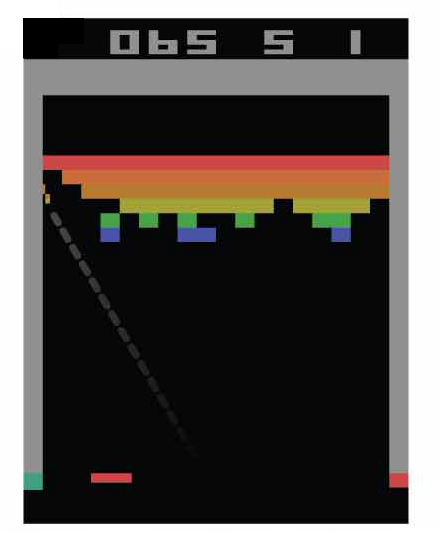
\includegraphics[width=0.25\textwidth]{breakout_frame}
\end{center}

\vspace{-\baselineskip}

{\small
V.~Mnih, K.~Kavukcuoglu, D.~Silver, \dots, D.~Hassabis. \emph{Human-level control through deep reinforcement learning.} Nature (2015) \nocite{Mnih2015}
}
\end{frame}



\begin{frame}
\frametitle{Policy gradient methods}
Idea: compute optimal policy $\pi^*: \mathsf{S} \to \mathsf{A}$ \emph{directly}, i.e., in general without computing value function $U(s)$ or Q-value function $Q(s, a)$ (model free, works for high-dimensional state spaces)

Ansatz for policy function: $\pi_{\theta}$, with to-be optimized parameters $\theta \in \R^m$, e.g., weights and bias vectors of an ANN

Use (as before) the expected utility to evaluate a policy function, with a default initial state $\hat{s}_0$:
\[
J(\theta) := U^{\pi_{\theta}}(\hat{s}_0) = \mathbb{E}\!\left[ \sum_{t=0}^\infty \gamma^t R(s_t) \Big\vert s_0 = \hat{s}_0, \pi_{\theta} \right]
\]
Goal: $\theta^* = \argmax_{\theta} J(\theta)$
\end{frame}



\begin{frame}
\frametitle{Policy gradient theorem}
In the following: policy function specifies action probabilities: $\pi(a \vert s)$ (instead of $a = \pi(s)$)

$\leadsto$ \textbf{policy gradient theorem} (see supplementary slides for derivation):
\[
\nabla J(\theta) = \mathbb{E}\!\left[ \sum_{t=0}^{\infty} \left(\sum_{t'=t}^{\infty} \gamma^{t'} R(s_{t'})\right) \nabla_{\theta} \log \pi_{\theta}(a_t \vert s_t) \big\vert \pi_{\theta} \right]
\]
Interpretation: to optimize $J(\theta)$ via gradient descent: if remaining ``cumulative discounted reward'' $\sum_{t'=t}^{\infty} \gamma^{t'} R(s_{t'})$ starting from $t$ is positive, then increase probability $\pi(a_t \vert s_t)$ of chosen actions
\end{frame}



\begin{frame}
\frametitle{REINFORCE algorithm}
Directly based on formula for $\nabla J(\theta)$: gradient descent with learning rate $\eta$

\begin{algorithmic}[1]
\State Chose initial parameters $\theta$
\For {$\text{episode} \gets 0, 1, \dots$}
    \State Run simulation using policy $\pi_{\theta}$, obtain trajectory $(s_0, a_0, r_0, \dots, s_T, a_T, r_T)$
    \For {$t \gets 0, 1, \dots, T$}
        \State $G_t \gets \sum_{t'=t}^T \gamma^{t'-t} \, r_{t'}$
        \State $\theta \gets \theta + \eta \, \gamma^t G_t \nabla_{\theta} \log \pi_{\theta}(a_t \vert s_t)$ \Comment{gradient step}
    \EndFor
\EndFor
\end{algorithmic}

Remarks:\\
\begin{itemize}
\item Variants of the algorithm without factor $\gamma^t$ in line $6$
\item Can apply gradient only ``a posteriori'', i.e., after completing a game
\end{itemize}

\vfill

{\small
R.~J.~Williams. \emph{Simple statistical gradient-following algorithms for connectionist reinforcement learning} (1992) \nocite{Williams1992}
}
\end{frame}



\begin{frame}
\frametitle{Actor critic method}
Motivation: reduce variance when estimating $\nabla J(\theta)$ via sampling
\begin{center}
\begin{tikzpicture}[>=stealth]
\draw[->] (0, 0) to (4, 0) node [right] {episode};
\draw[->] (0, 0) to (0, 3) node [above] {$\nabla J(\theta)$};
\draw[dashed] (0, 1.5) -- (4, 1.5);
\draw[<->] (4.2, 0.75) -- node [right] {large variance} (4.2, 2.25);
\draw[fill]
    (0.25, 1.58806) circle [radius=0.8pt]
    (0.5,  1.17362) circle [radius=0.8pt]
    (0.75, 1.79761) circle [radius=0.8pt]
    (1,    1.44665) circle [radius=0.8pt]
    (1.25, 0.80105) circle [radius=0.8pt]
    (1.5,  1.59561) circle [radius=0.8pt]
    (1.75, 1.06765) circle [radius=0.8pt]
    (2,    1.91863) circle [radius=0.8pt]
    (2.25, 1.67885) circle [radius=0.8pt]
    (2.5,  0.98468) circle [radius=0.8pt]
    (2.75, 1.74488) circle [radius=0.8pt]
    (3,    1.04269) circle [radius=0.8pt]
    (3.25, 1.85809) circle [radius=0.8pt]
    (3.5,  1.93423) circle [radius=0.8pt]
    (3.75, 1.08673) circle [radius=0.8pt]
    (4,    1.63758) circle [radius=0.8pt];
\end{tikzpicture}
\hspace{0.01\textwidth}
\begin{tikzpicture}[>=stealth]
\draw[->] (0, 0) to (4, 0) node [right] {episode};
\draw[->] (0, 0) to (0, 3) node [above] {$\nabla J(\theta)$};
\draw[dashed] (0, 1.5) -- (4, 1.5);
\draw[<->] (4.2, 1.25) -- node [right] {small variance} (4.2, 1.75);
\draw[fill]
    (0.25, 1.6046)  circle [radius=0.8pt]
    (0.5,  1.42427) circle [radius=0.8pt]
    (0.75, 1.41584) circle [radius=0.8pt]
    (1,    1.21055) circle [radius=0.8pt]
    (1.25, 1.52433) circle [radius=0.8pt]
    (1.5,  1.23628) circle [radius=0.8pt]
    (1.75, 1.64204) circle [radius=0.8pt]
    (2,    1.48314) circle [radius=0.8pt]
    (2.25, 1.42501) circle [radius=0.8pt]
    (2.5,  1.57837) circle [radius=0.8pt]
    (2.75, 1.57238) circle [radius=0.8pt]
    (3,    1.50746) circle [radius=0.8pt]
    (3.25, 1.80011) circle [radius=0.8pt]
    (3.5,  1.39314) circle [radius=0.8pt]
    (3.75, 1.4137)  circle [radius=0.8pt]
    (4,    1.44857) circle [radius=0.8pt];
\end{tikzpicture}
\end{center}

Idea: in derivation of the policy gradient theorem:
\[
\nabla J(\theta) = \sum_{t=0}^{\infty} \sum_{s \in \mathsf{S}} \mathbb{P}_{\theta}(\hat{s}_0 \to s \text{ in } t \text{ steps}) \gamma^t \sum_{a} Q^{\pi_{\theta}}(s, a) \nabla_{\theta} \pi_{\theta}(a \vert s):
\]
replace $\sum_{a} Q^{\pi_{\theta}}(s, a) \nabla_{\theta} \pi_{\theta}(a \vert s)$ by $\sum_{a} \left( Q^{\pi_{\theta}}(s, a) - b(s)\right) \nabla_{\theta} \pi_{\theta}(a \vert s)$ using an arbitrary ``baseline''-function $b: \mathsf{S} \to \R$: (only needs to be independent of parameters $\theta$)

Overall value remains unchanged, since
\[
\sum_{a} b(s) \nabla_{\theta} \pi_{\theta}(a \vert s) = b(s) \nabla_{\theta} \underbrace{\sum_{a} \pi_{\theta}(a \vert s)}_{= 1} = 0
\]
\end{frame}



\begin{frame}
\frametitle{Actor critic method, continued}
Leads to generalized formula for $\nabla J(\theta)$:
\[
\begin{split}
\nabla J(\theta)
&= \mathbb{E}\!\left[ \sum_{t=0}^{\infty} \gamma^{t} \left( \left(\sum_{t'=t}^{\infty} \gamma^{t'-t} R(s_{t'})\right) - b(s_t) \right) \nabla_{\theta} \log \pi_{\theta}(a_t \vert s_t) \Big\vert \pi_{\theta} \right] \\
&= \mathbb{E}\!\left[ \sum_{t=0}^{\infty} \gamma^{t} \Big( Q^{\pi_{\theta}}(s_t, a_t) - b(s_t) \Big) \nabla_{\theta} \log \pi_{\theta}(a_t \vert s_t) \Big\vert \pi_{\theta} \right]
\end{split}
\]

$\sum_{t'=t}^{\infty} \gamma^{t'-t} R(s_{t'}) - b(s_t)$: deviation of observed ``cumulative reward'' from baseline $\leadsto$ within gradient step: increase or decrease probability of chosen action depending on whether \emph{deviation} positive or negative

\medskip

Typical choice of $b(s)$: value function $U_{\phi}(s)$ with parameters $\phi$ (independent of $\theta$)

Deviation denoted \textbf{advantage}:
\[
A_t = Q^{\pi_{\theta}}(s_t, a_t) - U_{\phi}(s_t)
\]
\end{frame}



\begin{frame}
\frametitle{Actor critic method, continued}
$\leadsto$ \textbf{actor critic method}:\\
\begin{itemize}
\item actor: policy function $\pi_{\theta}$
\item critic: evaluation of chosen actions based on $A_t$
\end{itemize}\\
Parameters $\theta$ and $\phi$ are simultaneously optimized

Pseudo code (given learning rate $\eta$ and $\tilde{\eta}$):
\begin{algorithmic}[1]
\State Chose initial parameters $\theta$ and $\phi$
\For {$\text{episode} \gets 0, 1, \dots$}
    \State Run simulation using policy $\pi_{\theta}$, obtain trajectory $(s_0, a_0, r_0, \dots, s_T, a_T, r_T)$
    \For {$t \gets 0, 1, \dots, T$}
        \State $G_t \gets \sum_{t'=t}^T \gamma^{t'-t} \, r_{t'}$
        \State $A_t \gets G_t - U_{\phi}(s_t)$
        \State $\theta \gets \theta + \eta \, \gamma^t A_t \nabla_{\theta} \log \pi_{\theta}(a_t \vert s_t)$ \Comment{gradient step for $\theta$}
        \State $\phi \gets \phi + \tilde{\eta} A_t \nabla_{\phi} U_{\phi}(s_t)$ \Comment{gradient step for $\phi$}
    \EndFor
\EndFor
\end{algorithmic}

Remarks: typical asynchronous variants with multiple agents running in parallel cf.\ A3C (``asynchronous advantage actor critic'') \nocite{Mnih2016}
\end{frame}



\begin{frame}
\frametitle{Example: AlphaGo Zero}
\begin{center}
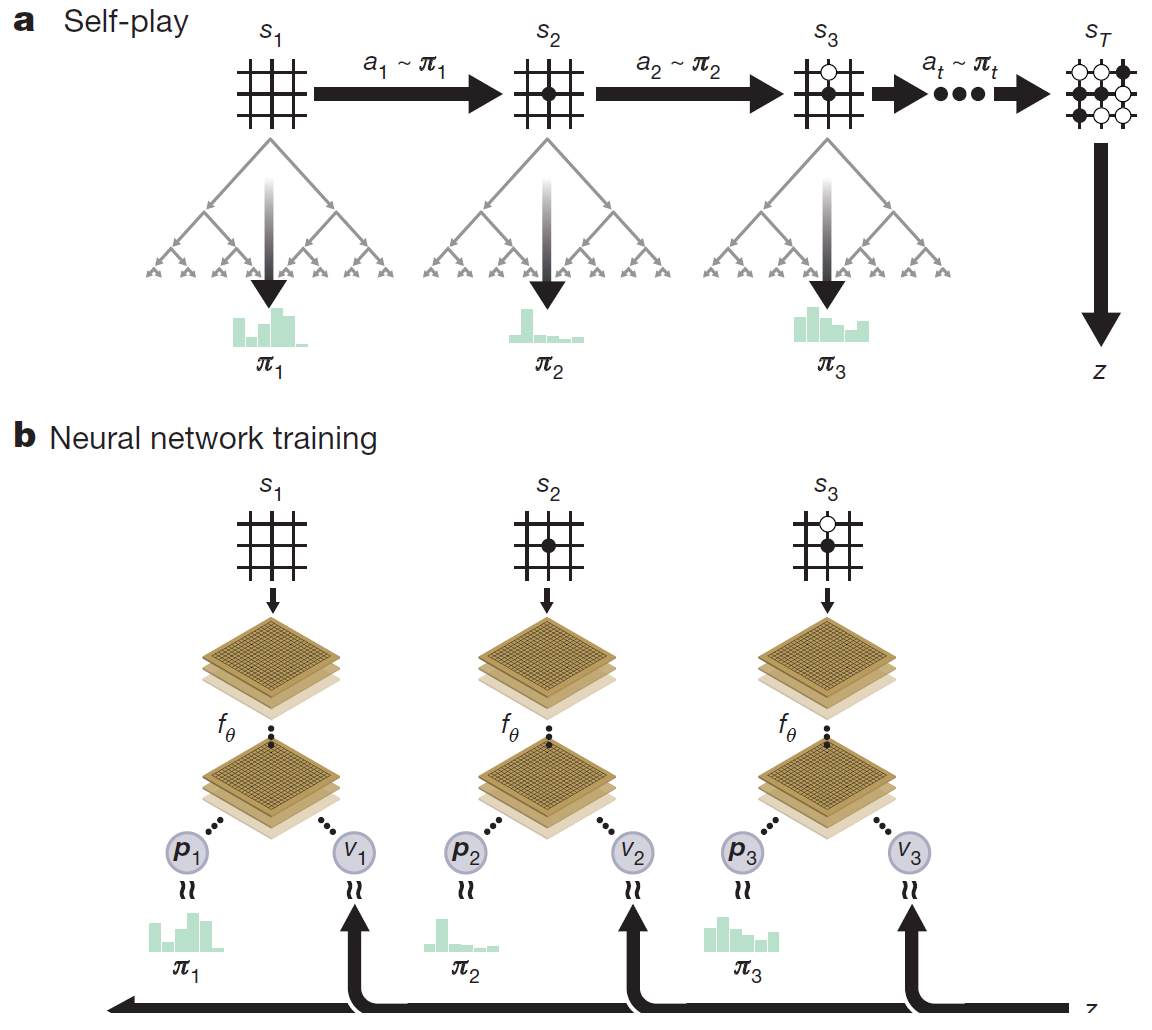
\includegraphics[width=0.6\textwidth]{AlphaGo_selfplay_training}
\end{center}

{\small
D.~Silver, \dots, D.~Hassabis. \emph{Mastering the game of Go without human knowledge.} Nature (2017) \nocite{AlphaGoZero2017}
}
\end{frame}



\PraesentationMasterWeissBlau
\begin{frame}
\frametitle{Hands-on example: simplified Pac-Man}
\href{https://github.com/cmendl/reinforcement-learning-course}{https://github.com/cmendl/reinforcement-learning-course}, subfolder \emph{code/}
\end{frame}
\PraesentationMasterStandard



\begin{frame}
\frametitle{Code structure}
\href{https://github.com/cmendl/reinforcement-learning-course}{https://github.com/cmendl/reinforcement-learning-course}, subfolder \emph{code/}
\begin{center}
\includegraphics[width=0.3\textwidth]{mdp_ghost_environment/mdp_ghost_environment}
\end{center}\\
\begin{itemize}
\item Iterative ``dynamic programming'' algorithms in \emph{mdp.py}
\item Environment: plain maze or maze with ghost in \emph{env.py}, \\
geometry specified in text files (like \emph{maze\_geometry.txt})
\item Policy gradient algorithm in \emph{pg.py}, corresponding (simple two-layer) network defined in \emph{policy\_net.py}
\item Demos as Jupyter notebooks
\end{itemize}
\end{frame}



\begin{frame}
\frametitle{References}
\printbibliography
\end{frame}



\PraesentationMasterWeissBlau
\begin{frame}
\frametitle{Supplementary slides}
\end{frame}
\PraesentationMasterStandard



\begin{frame}
\frametitle{Derivation of the policy gradient theorem}
Here generalization to probabilistic policy function: $\pi(a \vert s)$ (instead of $a = \pi(s)$)

Note that
\[
U^{\pi}(s) = \sum_{a \in \mathsf{A}} \pi(a \vert s) Q^{\pi}(s, a) \quad \forall s \in \mathsf{S}
\]
and
\[
Q^{\pi}(s, a) = R(s) + \gamma \sum_{s'} \mathbb{P}(s' \vert s, a) U^{\pi}(s') \quad \forall s \in \mathsf{S}, a \in \mathsf{A}.
\]
Therefore, combined with product rule:
\[
\begin{split}
\nabla_{\theta} U^{\pi_{\theta}}(s)
&= \sum_{a \in \mathsf{A}} \big( \nabla_{\theta} \pi_{\theta}(a \vert s) Q^{\pi_{\theta}}(s, a) + \pi_{\theta}(a \vert s) \nabla_{\theta} Q^{\pi_{\theta}}(s, a) \big) \\
&= \sum_{a} \nabla_{\theta} \pi_{\theta}(a \vert s) Q^{\pi_{\theta}}(s, a) + \gamma \sum_{s', a} \pi_{\theta}(a \vert s) \mathbb{P}(s' \vert s, a) \nabla_{\theta} U^{\pi_{\theta}}(s') \\
&= \sum_{a} \nabla_{\theta} \pi_{\theta}(a \vert s) Q^{\pi_{\theta}}(s, a) + \gamma \sum_{s'} \mathbb{P}_{\theta}(s' \vert s) \nabla_{\theta} U^{\pi_{\theta}}(s'),
\end{split}
\]
with
\[
\mathbb{P}_{\theta}(s' \vert s) = \sum_{a} \pi_{\theta}(a \vert s) \mathbb{P}(s' \vert s, a)
\]
the transition probability $s \to s'$ following policy $\pi_{\theta}$.
\end{frame}



\begin{frame}
\frametitle{Derivation of the policy gradient theorem, continued}
Equation for $\nabla_{\theta} U^{\pi_{\theta}}$ yields recursive relation; repeated application $\leadsto$
\[
\nabla J(\theta) = \nabla_{\theta} U^{\pi_{\theta}}(\hat{s}_0) = \sum_{t=0}^{\infty} \sum_{s \in \mathsf{S}} \mathbb{P}_{\theta}(\hat{s}_0 \to s \text{ in } t \text{ steps}) \gamma^t \sum_{a} \nabla_{\theta} \pi_{\theta}(a \vert s) Q^{\pi_{\theta}}(s, a)
\]
Rewrite last term:
\[
\begin{split}
\gamma^t \sum_{a} \nabla_{\theta} \pi_{\theta}(a \vert s) Q^{\pi_{\theta}}(s, a)
&= \gamma^t \sum_{a} \pi_{\theta}(a \vert s) Q^{\pi_{\theta}}(s, a) \nabla_{\theta} \log \pi_{\theta}(a \vert s) \\
&= \mathbb{E}_a\!\left[ \gamma^t Q^{\pi_{\theta}}(s, a) \nabla_{\theta} \log \pi_{\theta}(a \vert s) \big\vert \pi_{\theta} \right] \\
&= \mathbb{E}\!\left[ \sum_{t'=t}^{\infty} \gamma^{t'} R(s_{t'}) \nabla_{\theta} \log \pi_{\theta}(a_t \vert s_t) \big\vert s_t = s, \pi_{\theta} \right],
\end{split}
\]
with the expectation value referring to trajectories $(s_t, a_t, s_{t+1}, a_{t+1}, \dots)$ starting from time $t$.

In summary:
\[
\nabla J(\theta) = \mathbb{E}\!\left[ \sum_{t=0}^{\infty} \left(\sum_{t'=t}^{\infty} \gamma^{t'} R(s_{t'})\right) \nabla_{\theta} \log \pi_{\theta}(a_t \vert s_t) \big\vert \pi_{\theta} \right]
\]
\end{frame}



\end{document}
